\documentclass{tufte-handout}
\usepackage{../braph2_dev}
\usepackage{graphicx, booktabs, array}
%\geometry{showframe} % display margins for debugging page layout

\title{Implement a new Property Panel}

\begin{document}

\maketitle

\begin{abstract}
\noindent
This is the developer tutorial for implementing a new property panel. 
In this tutorial, we will explain how to create the generator file \fn{*.gen.m} for a new property panel which can then be compiled by \code{braph2genesis}, using the property panel \code{PanelPropLogical} as an example.
\end{abstract}

\tableofcontents

%%%%% %%%%% %%%%% %%%%% %%%%%
\clearpage
\section{Implementation of Property Panel (PanelPropLogical)}


We will start by implementing in detail the property panel \code{PanelPropLogical}, which applies the general concepts of a property panel and is a direct extension of the element \code{PanelProp}.

\begin{lstlisting}[
	label=cd:m:panelproplogical:header,
	caption={
		{\bf PanelPropLogical element header.}
		The \code{header} section of generator code for \fn{\_PanelPropLogical.gen.m} provides the general information about the \code{PanelPropLogical} element.
	}
]
%% ¡header!
PanelPropLogical < PanelProp (pr, panel property logical) plots the panel of a property logical.  ¥\circled{1}\circlednote{1}{The element \code{PanelPropLogical} is defined as a subclass of \code{PanelProp}. The moniker will be \code{pr}.}¥

%%% ¡description!
PanelPropLogical plots the panel for a LOGICAL property with a checkbox.
It works for all categories.

\end{lstlisting}

\begin{lstlisting}[
	label=cd:m:panelproplogical:props_update,
	caption={
		{\bf PanelPropLogical element props update.}
		The \code{props\_update} section of generator code for \fn{\_PanelPropLogical.gen.m} updates the properties of the \code{PanelProp} element. This defines the core properties of the property panel.
	}
]
%% ¡props_update!

...

%%% ¡prop!
EL (data, item) is the element. ¥\circled{2}\circlednote{2}{It defines the element for this property panel.}¥
%%%% ¡default!
PanelProp()

%%% ¡prop!
PROP (data, scalar) is the property number. ¥\circled{3}\circlednote{3}{It defines the property pointer associated with the element for this property panel.}¥
%%%% ¡default!
PanelProp.DRAW

...

\end{lstlisting}

\begin{lstlisting}[
	label=cd:m:panelproplogical:props,
	caption={
		{\bf PanelPropLogical new props.}
		The \code{props} section of generator code for \fn{\_PanelPropLogical.gen.m} defines the graphical elements for the \code{PanelPropLogical} element.
	}
]
%% ¡props!

%%% ¡prop!
CHECKBOX (evanescent, handle) is the logical value checkbox.  ¥\circled{4}\circlednote{4}{The panel for a property logical has a \code{CHECKBOX}.}¥
%%%% ¡calculate!
el = pr.get('EL');
prop = pr.get('PROP');

checkbox = uicheckbox( ...
    'Parent', pr.memorize('H'), ... % H = p for Panel
    'Tag', 'CHECKBOX', ...
    'Text', '', ...
    'FontSize', BRAPH2.FONTSIZE, ...
    'Tooltip', [num2str(el.getPropProp(prop)) ' ' el.getPropDescription(prop)], ...
    'ValueChangedFcn', {@cb_checkbox} ...
    );

value = checkbox;
%%%% ¡calculate_callbacks!
function cb_checkbox(~, ~) ¥\circled{5}\circlednote{5}{The panel for a property logical has a \code{callbacks} for its \code{CHECKBOX}, defining the appropreate behavior of the checkbox.}¥
    el = pr.get('EL');
    prop = pr.get('PROP'); ¥\circled{6}\circlednote{6}{The \code{callback} firstly extracts the property logical.}¥
    
    checkbox = pr.get('CHECKBOX');
    new_value = logical(get(checkbox, 'Value'));  ¥\circled{7}\circlednote{7}{The \code{callback} then extracts the value of the \code{CHECKBOX} as a new value.}¥
    
    el.set(prop, new_value)  ¥\circled{8}\circlednote{8}{Finally, the \code{callback} sets the new value to the logical property.}¥
end

\end{lstlisting}

\begin{lstlisting}[
	label=cd:m:panelproplogical:props_update2,
	caption={
		{\bf PanelPropLogical element props update.}
		The continuing \code{props\_update} section of generator code for \fn{\_PanelPropLogical.gen.m} updates the rest of the properties of the \code{PanelProp} element. This defines the panel drawing of the property panel.
	}
]
%% ¡props_update!

...


%%% ¡prop!
X_DRAW (query, logical) draws the property panel.  ¥\circled{9}\circlednote{9}{\code{X\_DRAW} draws the panel. In this case, the panel contains a \code{CHECKBOX}.}¥

%%%% ¡calculate!
value = calculateValue@PanelProp(pr, PanelProp.X_DRAW, varargin{:}); % also warning
if value
    pr.memorize('CHECKBOX')
end

%%% ¡prop!
DELETE (query, logical) resets the handles when the panel is deleted. ¥\circled{10}\circlednote{10}{\code{DELETES} resets the handles when the panel is deleted. In this case, it sets the \code{CHECKBOX} to \code{NoValue()}.}¥
%%%% ¡calculate!
value = calculateValue@PanelProp(pr, PanelProp.DELETE, varargin{:}); % also warning
if value
    pr.set('CHECKBOX', Element.getNoValue())
end

%%% ¡prop!
HEIGHT (gui, size) is the pixel height of the property panel. ¥\circled{11}\circlednote{11}{\code{HEIGHT} specifies the height of the panel that contains the \code{CHECKBOX}.}¥
%%%% ¡default!
s(4)

%%% ¡prop!
REDRAW (query, logical) resizes the property panel and repositions its graphical objects.
%%%% ¡calculate!
value = calculateValue@PanelProp(pr, PanelProp.REDRAW, varargin{:}); % also warning
if value
    w_p = get_from_varargin(w(pr.get('H'), 'pixels'), 'Width', varargin);
    
    set(pr.get('CHECKBOX'), 'Position', [s(.3) s(.3) .70*w_p s(1.75)])
end    

%%% ¡prop!
UPDATE (query, logical) updates the content and permissions of the editfield. ¥\circled{12}\circlednote{12}{\code{UPDATE} updates the status of the \code{CHECKBOX} based on various scenario, influenced by the property's category.}¥
%%%% ¡calculate!
value = calculateValue@PanelProp(pr, PanelProp.UPDATE, varargin{:}); % also warning
if value

    el = pr.get('EL');
    prop = pr.get('PROP');
    
    switch el.getPropCategory(prop)
        case Category.CONSTANT ¥\circled{13}\circlednote{13}{When the property is a \code{CONSTANT}, the \code{CHECKBOX} is disabled as it cannot be changed.}¥
            set(pr.get('CHECKBOX'), ...
                'Value', el.get(prop), ...
                'Enable', 'off' ...
                )

        case Category.METADATA ¥\circled{14}\circlednote{14}{When the property is a \code{METADATA}, the \code{CHECKBOX}'s enabling status corresponds to whether it is locked.}¥
            set(pr.get('CHECKBOX'), 'Value', el.get(prop))

            if el.isLocked(prop)
                set(pr.get('CHECKBOX'), 'Enable', 'off')
            end
            
        case {Category.PARAMETER, Category.DATA, Category.FIGURE, Category.GUI}  ¥\circled{15}\circlednote{15}{The behavior of the \code{CHECKBOX} varies according to different categories, as we have seen two examples until this point. To ensure precise control over the \code{CHECKBOX}'s functionality, consider the specific cases for behavior.}¥
            set(pr.get('CHECKBOX'), 'Value', el.get(prop))

            prop_value = el.getr(prop);
            if el.isLocked(prop) || isa(prop_value, 'Callback')
                set(pr.get('CHECKBOX'), 'Enable', 'off')
            end
            
        case {Category.RESULT Category.QUERY Category.EVANESCENT}
            prop_value = el.getr(prop);

            if isa(prop_value, 'NoValue')
                set(pr.get('CHECKBOX'), 'Value', el.getPropDefault(prop))
            else
                set(pr.get('CHECKBOX'), 'Value', el.get(prop))
            end
            
            set(pr.get('CHECKBOX'), 'Enable', 'off')
    end
end

\end{lstlisting}



%%%%% %%%%% %%%%% %%%%% %%%%%
\clearpage

\section{Property Panel for all User Interface Objects}

The concept of implementing PanelPropLogical, as shown in the previous section, can be seamlessly extended to all other user interface (UI) elements.

The subsequent table presents a comprehensive overview of various UI objects in BRAPH 2, each coupled with its corresponding property panel as an example.

\newcommand{\addpicbutton}{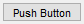
\includegraphics[width=6em]{fig01.png}}
\newcommand{\addpiccheckbox}{
\includegraphics[width=6em]{fig02.png}}
\newcommand{\addpiceditfield}{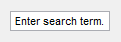
\includegraphics[width=6em]{fig03.png}}
\newcommand{\addpicslider}{
\includegraphics[width=6em]{fig04.png}}
\newcommand{\addpiclistbox}{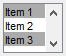
\includegraphics[width=6em]{fig05.png}}
\newcommand{\addpicdropdown}{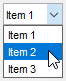
\includegraphics[width=6em]{fig06.png}}
\newcommand{\addpictextarea}{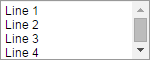
\includegraphics[width=6em]{fig07.png}}
\newcommand{\addpiccontextmenu}{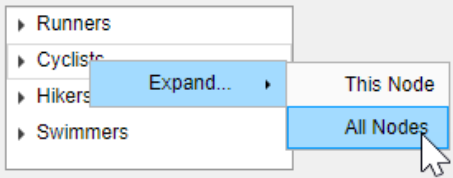
\includegraphics[width=6em]{fig08.png}}
\newcommand{\addpictable}{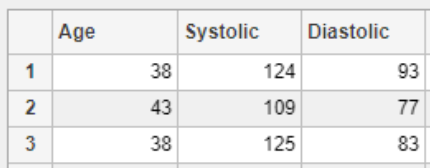
\includegraphics[width=6em]{fig09.png}}
\newcolumntype{C}{>{\centering\arraybackslash}m{6em}}
\begin{table}\sffamily
	\begin{tabular}{l*4{C}@{}}
		\toprule
		UI Object & Example & PanelProp Element \\ 
		\midrule
		uibutton & \addpicbutton & PanelPropItem \\ 
		checkbox & \addpiccheckbox & PanelPropLogical \\ 
		uitextarea  & \addpictextarea & PanelPropStringList \\
		uieditfield & \addpiceditfield & PanelPropString \\
		uidropdown & \addpicdropdown & PanelPropLogical \\
		uicontextmenu & \addpiccontextmenu & PanelPropMatrix \\
		uitable & \addpictable & PanelPropItemList \\
		uilistbox & \addpiclistbox & PanelPropClassList \\
		uislider & \addpicslider & PanelPropCell \\
		\bottomrule \\
	\end{tabular}
\end{table} 
By referencing the related PanelProp elements, the process of creating a new property panel becomes straightforward and efficient.


%\bibliography{biblio}
%\bibliographystyle{plainnat}

\end{document}